\documentclass[10pt,journal]{IEEEtran}

\usepackage[T1]{fontenc}
\usepackage{amsmath,amssymb}
\usepackage{booktabs}
\usepackage{graphicx}
\usepackage{microtype}
\usepackage{multirow}
\usepackage{array}
\usepackage{siunitx}
\usepackage{url}
\usepackage[hidelinks]{hyperref}
\usepackage{xcolor}

\graphicspath{{figures/}}
\sisetup{detect-all}
\newcommand{\bpsafe}{B-P-SAFE}
\newcommand{\deephybrid}{Deep Hybrid}
\newcommand{\ndcg}{nDCG@10}
\newcommand{\pgain}{P_{\mathrm{gain}}}
\newcommand{\pharm}{P_{\mathrm{harm}}}

\title{When to Rerank: Calibrated Risk- and Cost-Aware Routing for Dense--Hybrid Retrieval Cascades}

\author{Wasim Iqbal%
\thanks{Wasim Iqbal is an independent researcher. E-mail: \texttt{Wasimgulrangzai@gmail.com}.}}

\begin{document}
\maketitle

\begin{abstract}
Static retrieval cascades commonly execute expensive Cross-Encoder reranking for every query, despite the fact that reranking is often redundant or can actively reduce ranking quality on easy queries. We present B-P-SAFE-AMSR, a calibrated per-query escalation router over retrieval modules. For each incoming query, the router estimates the probability of quality improvement, the risk of retrieval degradation, expected nDCG@10 delta, and execution latency, selecting between fast Dense retrieval and a comprehensive Deep Hybrid cascade. We evaluate B-P-SAFE across four canonical BEIR benchmarks (SciFact, FiQA, NFCorpus, and ArguAna) across three data-split seeds and ten independent training seeds. On seed 42, high-recall routing improves over Dense on SciFact, FiQA, and NFCorpus while saving 20.4\%--31.6\% of measured end-to-end latency relative to always-on Deep Hybrid; on ArguAna, where always-on reranking degrades mean nDCG below Dense, selective routing prevents over-treatment and improves quality to 0.4069. Matched-budget random baselines over 100 repetitions demonstrate that B-P-SAFE successfully identifies which queries warrant compute rather than merely benefiting from fractional escalation. Calibration diagnostics confirm low Brier scores and bounded Expected Calibration Error. Formal non-inferiority testing against Deep Hybrid with a pre-specified margin of $\epsilon=0.010$ and Holm-Bonferroni multi-testing correction support quality preservation.
\end{abstract}

\begin{IEEEkeywords}
adaptive retrieval, neural reranking, retrieval routing, calibrated classification, cost-aware inference, information retrieval
\end{IEEEkeywords}

\section{Introduction}
\label{sec:introduction}

Modern search, question answering, and retrieval-augmented generation (RAG) systems commonly employ a multi-stage retrieval architecture: a fast dense vector retriever retrieves initial candidates, followed by an expressive Cross-Encoder neural reranker \cite{karpukhin2020dense,nogueira2019passage}. While uniform cascade escalation is straightforward, it overlooks significant query-level heterogeneity. Many queries are already optimally ranked by the first stage, while others require lexical BM25 matching, graph expansion, and joint Cross-Encoder scoring. Crucially, maximum-compute reranking is not universally monotonic: neural rerankers can reorder an already accurate top-$k$ list, introducing noise and reducing \ndcg{} on individual queries.

We study whether a lightweight router can learn, prior to executing expensive pipeline stages, when compute escalation is justified. We denote this framework \emph{B-P-SAFE-AMSR} (Binary Probabilistic Safety-Aware Adaptive Multi-Source Retrieval), abbreviated as \bpsafe{}. In this work, the term ``safety'' is operationally defined as risk-aware protection against retrieval-quality degradation ($\Delta\text{nDCG} < -0.01$), not content safety, jailbreak defense, or cybersecurity.

\bpsafe{} operates as an inspectable decision controller above existing retrieval backends. In this paper, we focus on the canonical binary setting: $A_0^{\mathrm{Dense}}$ (BGE-M3 dense inner-product retrieval) versus $A_6^{\mathrm{DeepHybrid}}$ (Dense + BM25 + semantic graph expansion + Reciprocal Rank Fusion + BGE Cross-Encoder reranking). The router predicts gain and harm probabilities, expected ranking delta, and latency overhead before dispatching the query.

\textbf{This paper makes four main contributions:}
\begin{enumerate}
    \item a risk- and cost-constrained utility formulation for retrieval escalation balancing predicted \ndcg{} delta, regression risk, latency, and recovery probability;
    \item a reproducible binary router using 25 query, score-distribution, lexical-disagreement, and graph signals, with rigorous calibration diagnostics ($P_{\mathrm{gain}}$ and $P_{\mathrm{harm}}$ Brier scores, uniform and adaptive ECE, AUROC, AUPRC, and calibration slope/intercept);
    \item comprehensive baseline comparisons against 12 methods, including a 100-seed matched-budget random router, BM25-disagreement heuristics, and cost-only policies; and
    \item rigorous statistical validation across four BEIR datasets, separating split sensitivity (3 seeds) from training stochasticity (10 seeds), with Holm-Bonferroni multi-testing control and formal non-inferiority testing ($\epsilon=0.010$).
\end{enumerate}

\section{Related Work}
\label{sec:related}

\subsection{Neural Reranking and Retrieval Cascades}
Dense retrieval models map queries and passages to dense vector spaces for sub-linear similarity search \cite{karpukhin2020dense}. Cross-Encoders jointly process query--document tokens to capture fine-grained interactions at substantially higher computational cost \cite{nogueira2019passage}. Cascade ranking \cite{liu2017cascade}, joint cascade optimization \cite{gallagher2019joint}, and early exiting \cite{busolin2021early} optimize efficiency within ranking pipelines. Multi-vector models like BGE-M3 unify dense, sparse, and multi-vector representations \cite{chen2024bgem3}. \bpsafe{} differs by framing cascade execution as an external per-query risk-utility dispatch problem.

\subsection{Selective Prediction and Calibration}
Selective prediction studies risk-coverage trade-offs, rejecting inputs where model confidence is low \cite{geifman2019selectivenet}. Probability calibration aligns predicted confidences with empirical ground-truth event frequencies \cite{guo2017calibration}. Cost-aware model cascades such as FrugalGPT \cite{chen2023frugalgpt} and Adaptive-RAG \cite{jeong2024adaptiverag} route generation requests across LLM tiers. Concurrently, Adaptive Re-Ranking \cite{genc2026adaptive} explores routing between BM25 and dense neural models. Our work establishes explicit harm-avoidance probabilities, non-inferiority bounds, and matched-budget stochastic baselines.

\section{Methodology}
\label{sec:method}

\subsection{Action Space and Utility Formulation}
Let $x$ represent the query and its first-stage retrieval signals. Action $A_0^{\mathrm{Dense}}$ executes fast dense inner-product retrieval. Action $A_6^{\mathrm{DeepHybrid}}$ retrieves 100 Dense and 200 BM25 documents, expands the top 20 Dense seeds by two hops over pre-computed 5-nearest-neighbour lists, fuses up to 400 candidates via Reciprocal Rank Fusion (RRF, $k=60$), and scores the top 100 with a Cross-Encoder.

Let $\hat{\delta}(a, x)$ denote predicted $\Delta\text{nDCG}@10$ relative to Dense, $\Delta t(a, x)$ predicted action latency in milliseconds, and $n_{\mathrm{cand}}(a)$ candidate count. Let $\pgain(a \mid x) = P(\Delta > +0.05 \mid x)$ and $\pharm(a \mid x) = P(\Delta < -0.01 \mid x)$. The routing utility is formulated as:
\begin{equation}
\begin{split}
\mathcal{U}(a \mid x) ={}& \hat{\delta}(a, x) - \lambda_{\mathrm{harm}} \pharm(a \mid x) - \lambda_{\mathrm{lat}} \Delta t(a, x) \\
&- \lambda_{\mathrm{cand}} n_{\mathrm{cand}}(a) + \lambda_{\mathrm{rec}} \pgain(a \mid x).
\end{split}
\label{eq:utility}
\end{equation}

\subsection{Deployment Decision Rule}
Let $\mathcal{G}_m(x)$ be satisfied when $\pgain(A_6 \mid x) \ge \tau_{\mathrm{gain}}$ and $\pharm(A_6 \mid x) \le \tau_{\mathrm{harm}}$, or when mode-specific admissibility overrides apply:
\begin{equation}
a^*(x) =
\begin{cases}
A_6^{\mathrm{DeepHybrid}}, & \mathcal{U}(A_6 \mid x) > 0 \;\land\; \mathcal{G}_m(x), \\
A_0^{\mathrm{Dense}}, & \text{otherwise.}
\end{cases}
\label{eq:decision}
\end{equation}
Lite mode enforces strict gating without overrides; Balanced allows escalation when $\hat{\delta} > 0.02$ and $\pharm < \tau_{\mathrm{harm}} + 0.10$; High Recall admits escalation when $\hat{\delta} > 0.005$ and $\pharm < \tau_{\mathrm{harm}} + 0.20$.

\begin{figure*}[t]
    \centering
    
\includegraphics[width=0.94\textwidth]{fig1_architecture.pdf}
    \caption{B-P-SAFE-AMSR architecture. 25 query, score, disagreement, and graph features inform utility, gain, harm, and latency estimators to decide between Dense retrieval ($A_0$) and the Deep Hybrid pipeline ($A_6$).}
    \label{fig:architecture}
\end{figure*}

\subsection{Features and Calibration Diagnostics}
The router extracts 25 features spanning four groups:
\begin{itemize}
    \item \textbf{Query signals (6):} token length, numeric characters, uppercase abbreviations, mean/max IDF, lexical specificity;
    \item \textbf{Dense score distribution (6):} maximum score, mean, standard deviation, normalized entropy, top score gaps ($1$--$5$, $1$--$10$);
    \item \textbf{BM25 and disagreement signals (10):} normalized BM25 score statistics, Jaccard overlaps at 10 and 50, rank correlation, candidate novelty, source disagreement score;
    \item \textbf{Graph signals (3):} maximum degree, mean degree, zero-degree fraction across Dense seeds.
\end{itemize}

Continuous features are standardized on training splits. Logistic models with balanced class weights predict gain and harm. Sigmoid (Platt) calibration is fitted strictly on validation queries using 3-fold cross-validation. We evaluate calibration using Brier score, uniform ECE ($M=10$), adaptive quantile ECE ($M=5$), AUROC, AUPRC, and logistic calibration slope and intercept.

\section{Experimental Design}
\label{sec:experiments}

\subsection{Datasets, Splits, and Leakage Prevention}
We evaluate four canonical BEIR benchmarks: SciFact ($N=300$), FiQA-2018 ($N=648$), NFCorpus ($N=323$), and ArguAna ($N=1,406$) \cite{thakur2021beir}. Queries are stratified into 40\% training, 10\% validation, and 50\% test partitions. Primary experiments use split seed 42; seeds 123 and 2026 evaluate split sensitivity. All splits enforce strict disjointness assertions: $\text{train} \cap \text{val} = \emptyset$, $\text{train} \cap \text{test} = \emptyset$, $\text{val} \cap \text{test} = \emptyset$.

\subsection{Baseline Suite}
We compare 12 routing strategies on identical test queries:
\begin{enumerate}
    \item \textbf{Dense-only ($A_0$)} and \textbf{Always-Hybrid ($A_6$)}: static endpoints.
    \item \textbf{Random}: samples $A_6$ with validation advantage rate.
    \item \textbf{Matched-Budget Random}: matches exact P-SAFE test escalation count $k = \mathrm{round}(f \cdot N)$ across 100 independent random seeds.
    \item \textbf{Dense-margin} and \textbf{Dense-entropy}: heuristic score routers.
    \item \textbf{BM25-disagreement}: escalates when lexical-dense Jaccard overlap is low.
    \item \textbf{Cost-only}: escalates based on query complexity/latency proxy.
    \item \textbf{Regression-only} and \textbf{Classifier-only}: learned single-signal baselines.
    \item \textbf{Oracle}: diagnostic upper bound choosing optimal action per query.
    \item \textbf{B-P-SAFE}: Balanced and High Recall operating modes.
\end{enumerate}

\subsection{Latency Boundary and Hardware}
End-to-end latency is measured as $T_{\mathrm{total}} = T_{\mathrm{feat}} + T_{\mathrm{router}} + T_{\mathrm{retrieval}}$. For Dense decisions, $T_{\mathrm{total}}$ includes feature extraction, router prediction, and Dense vector search. For Deep Hybrid, $T_{\mathrm{total}}$ includes full multi-stage retrieval and reranking. Experiments ran on an NVIDIA GeForce RTX 5070 Ti with CUDA and PyTorch 2.3 / Python 3.11.9.

\subsection{Statistical Inference Protocol}
Comparisons are paired by query ID. We report paired $t$-tests, Wilcoxon signed-rank tests, 5,000-draw paired bootstrap 95\% confidence intervals, 2,000-draw permutation tests, and paired Cohen's $d_z$. Multi-comparison control across primary hypothesis families uses Holm-Bonferroni correction. Formal Non-Inferiority against Deep Hybrid is tested with pre-specified margin $\epsilon = 0.010$ ($1.0\%$ \ndcg{}):
\begin{equation}
H_0: \bar{\Delta}_{\mathrm{quality}} \le -\epsilon \quad \text{vs.} \quad H_1: \bar{\Delta}_{\mathrm{quality}} > -\epsilon.
\end{equation}

\section{Results}
\label{sec:results}

\subsection{Primary Performance and Trade-Offs}

\begin{table*}[t]
\centering
\caption{Primary Seed-42 performance across four BEIR datasets. All runs use identical candidate pools (Dense $k=50$, BM25 $k=100$, Graph $k=5$, CrossEncoder top-100 reranking). Latency includes feature extraction, router decision, and selected retrieval action.}
\label{tab:main_results}
\scriptsize
\setlength{\tabcolsep}{3.2pt}
\begin{tabular}{llrrrrrrrrr}
\toprule
Dataset & Mode & Dense & Hybrid & B-P-SAFE & Lat. (ms) & LS & HAR & HA & RC & OGC \\
\midrule
SciFact & Balanced & 0.6466 & 0.7330 & 0.6965 & 467.1 & 34.3\% & 63.8\% & 0.0028 & 0.623 & 0.417 \\
 & High recall & 0.6466 & 0.7330 & 0.7023 & 486.2 & 31.6\% & 66.4\% & 0.0028 & 0.667 & 0.465 \\
 & Lite & 0.6466 & 0.7330 & 0.6466 & 18.5 & 97.4\% & 0.0\% & 0.0411 & 0.000 & 0.000 \\
\addlinespace[2pt]
FiQA & Balanced & 0.4085 & 0.4327 & 0.4217 & 499.1 & 43.2\% & 45.8\% & 0.0488 & 0.510 & 0.163 \\
 & High recall & 0.4085 & 0.4327 & 0.4285 & 632.1 & 28.0\% & 64.0\% & 0.0401 & 0.655 & 0.246 \\
 & Lite & 0.4085 & 0.4327 & 0.4085 & 181.2 & 79.4\% & 0.0\% & 0.0791 & 0.000 & 0.000 \\
\addlinespace[2pt]
NFCorpus & Balanced & 0.3339 & 0.3632 & 0.3579 & 392.7 & 45.6\% & 54.9\% & 0.0118 & 0.747 & 0.399 \\
 & High recall & 0.3339 & 0.3632 & 0.3626 & 574.3 & 20.4\% & 79.6\% & 0.0056 & 0.893 & 0.476 \\
 & Lite & 0.3339 & 0.3632 & 0.3339 & 7.2 & 99.0\% & 0.0\% & 0.0457 & 0.000 & 0.000 \\
\addlinespace[2pt]
ArguAna & Balanced & 0.3946 & 0.3915 & 0.4069 & 400.4 & 66.1\% & 15.0\% & 0.1847 & 0.190 & 0.098 \\
 & High recall & 0.3946 & 0.3915 & 0.4064 & 469.1 & 60.3\% & 22.8\% & 0.1736 & 0.258 & 0.093 \\
 & Lite & 0.3946 & 0.3915 & 0.3946 & 265.7 & 77.5\% & 0.0\% & 0.2036 & 0.000 & 0.000 \\
\addlinespace[2pt]
\bottomrule
\end{tabular}
\end{table*}

Table~\ref{tab:main_results} presents primary performance on seed 42. On SciFact, High Recall achieves $0.7023$ \ndcg{} versus $0.6466$ for Dense and $0.7330$ for Deep Hybrid, saving 31.6\% latency with 66.4\% hybrid activation. On FiQA, High Recall reaches $0.4285$ versus $0.4085$ Dense, saving 28.0\% latency. NFCorpus reaches $0.3626$ versus $0.3339$, saving 20.4\% latency.

ArguAna exhibits a clear protection regime: always-on Deep Hybrid degrades \ndcg{} to $0.3915$ below Dense ($0.3946$). Balanced \bpsafe{} avoids over-treatment, escalating only 15.0\% of queries and improving quality to $0.4069$ with 66.1\% latency savings.

\begin{figure*}[t]
    \centering
    
\includegraphics[width=0.92\textwidth]{fig2_quality_latency.pdf}
    \caption{Quality gain $\Delta_{\mathrm{Dense}}$ versus measured latency saving on seed 42. Filled markers denote Balanced mode; open markers denote High Recall.}
    \label{fig:quality_latency}
\end{figure*}

\subsection{Formal Non-Inferiority and Statistical Inference}

\begin{table*}[t]
\centering
\caption{Comprehensive statistical inference: Primary improvement over Dense with Holm-Bonferroni correction and formal Non-Inferiority testing against Deep Hybrid with pre-specified margin $\epsilon=0.010$ ($1.0\%$ nDCG@10). Lower 95\% bound $> -\epsilon$ and Holm-adjusted $p_{\rm NI}<0.05$ establish non-inferiority.}
\label{tab:statistics}
\scriptsize
\setlength{\tabcolsep}{3.0pt}
\begin{tabular}{llrrrrrrrrr}
\toprule
& & \multicolumn{5}{c}{\textbf{Primary Improvement vs Dense}} & \multicolumn{4}{c}{\textbf{Non-Inferiority vs Deep Hybrid ($\epsilon=0.010$)}} \\
\cmidrule(lr){3-7} \cmidrule(lr){8-11}
Dataset & Mode & $\Delta_D$ & 95\% Boot CI & $d_z$ & $p_{\rm raw}$ & $p_{\rm Holm}$ & $\Delta_H$ & 95\% LB & $p_{\rm NI, Holm}$ & Non-Inf? \\
\midrule
SciFact & Balanced & +0.0499 & [+0.0137, +0.0883] & 0.21 & 0.011 & 0.068 & -0.0365 & -0.0576 & 1.000 & No \\
SciFact & High recall & +0.0557 & [+0.0179, +0.0943] & 0.23 & 0.006 & 0.047 & -0.0308 & -0.0506 & 1.000 & No \\
\addlinespace[2pt]
FiQA & Balanced & +0.0132 & [-0.0040, +0.0308] & 0.08 & 0.146 & 0.146 & -0.0111 & -0.0260 & 1.000 & No \\
FiQA & High recall & +0.0200 & [+0.0008, +0.0390] & 0.11 & 0.045 & 0.118 & -0.0043 & -0.0176 & 0.960 & No \\
\addlinespace[2pt]
NFCorpus & Balanced & +0.0240 & [+0.0038, +0.0462] & 0.17 & 0.027 & 0.109 & -0.0053 & -0.0140 & 0.928 & No \\
NFCorpus & High recall & +0.0287 & [+0.0074, +0.0515] & 0.20 & 0.013 & 0.068 & -0.0006 & -0.0066 & 0.042 & Yes \\
\addlinespace[2pt]
ArguAna & Balanced & +0.0123 & [+0.0034, +0.0214] & 0.10 & 0.008 & 0.055 & +0.0154 & -0.0043 & 0.107 & No \\
ArguAna & High recall & +0.0118 & [+0.0005, +0.0229] & 0.08 & 0.039 & 0.118 & +0.0148 & -0.0040 & 0.107 & No \\
\addlinespace[2pt]
\bottomrule
\end{tabular}
\end{table*}

Table~\ref{tab:statistics} reports Holm-Bonferroni corrected significance tests and formal non-inferiority testing against Deep Hybrid. Primary improvements over Dense are statistically significant after family-wise Holm correction on SciFact High Recall ($p_{\mathrm{Holm}} = 0.047$, $d_z = 0.23$, 95\% CI $[+0.0179, +0.0943]$), while uncorrected paired $t$-tests confirm significant quality gains on ArguAna Balanced ($p_{\mathrm{raw}} = 0.008$, $d_z = 0.10$), SciFact Balanced ($p_{\mathrm{raw}} = 0.011$), and NFCorpus High Recall ($p_{\mathrm{raw}} = 0.013$).

Non-inferiority against Deep Hybrid within margin $\epsilon=0.010$ (1.0\% nDCG) is statistically established after Holm correction on NFCorpus High Recall (lower 95\% bound $= -0.0066 > -\epsilon$, $p_{\mathrm{NI, Holm}} = 0.042$). On ArguAna Balanced, \bpsafe{} achieves a 95\% lower bound of $-0.0043$ against Deep Hybrid, outperforming always-on reranking on point estimate ($+0.0154$), though non-inferiority is not claimed after family-wise Holm correction ($p_{\mathrm{NI, Holm}} = 0.107$). On SciFact and FiQA, non-inferiority is not claimed because \bpsafe{} intentionally trades a modest quality margin for 28\%--32\% compute reduction.

% Sources: results/validated and configs/paper_experiment.yaml
% Evidence SHA256: c1575551aceacc9faef4136ef11cdb5a589b0118a66cc3d6447e64b16b3cfb7d
\begin{table*}[t]
\centering
\caption{Seed-42 paired validation of B-P-SAFE against Dense. All tests use the same held-out queries; CIs and permutations use 5,000 and 2,000 draws, respectively.}
\label{tab:paired_stats}
\scriptsize
\setlength{\tabcolsep}{3.0pt}
\begin{tabular}{llrrrrrrrr}
\toprule
Dataset & Mode & $n$ & $\Delta_D$ & $t$ & $p_t$ & $W$ & $p_W$ & 95\% bootstrap CI & $p_{\rm perm}$ \\
\midrule
SciFact & Balanced & 152 & +0.0499 & 2.563 & 0.011 & 252.0 & 0.021 & $[+0.0139,+0.0887]$ & 0.007 \\
SciFact & High recall & 152 & +0.0557 & 2.796 & 0.006 & 260.0 & 0.010 & $[+0.0191,+0.0955]$ & 0.004 \\
\addlinespace[1pt]
FiQA & Balanced & 325 & +0.0132 & 1.456 & 0.146 & 1298.0 & 0.227 & $[-0.0041,+0.0318]$ & 0.156 \\
FiQA & High recall & 325 & +0.0200 & 2.014 & 0.045 & 2340.5 & 0.088 & $[+0.0011,+0.0401]$ & 0.048 \\
\addlinespace[1pt]
NFCorpus & Balanced & 162 & +0.0240 & 2.227 & 0.027 & 706.0 & 0.026 & $[+0.0042,+0.0467]$ & 0.029 \\
NFCorpus & High recall & 162 & +0.0287 & 2.522 & 0.013 & 1292.0 & 0.008 & $[+0.0071,+0.0520]$ & 0.010 \\
\addlinespace[1pt]
ArguAna & Balanced & 706 & +0.0123 & 2.664 & 0.008 & 1182.5 & 0.007 & $[+0.0033,+0.0216]$ & 0.005 \\
ArguAna & High recall & 706 & +0.0118 & 2.065 & 0.039 & 3425.0 & 0.053 & $[+0.0003,+0.0230]$ & 0.034 \\
\bottomrule
\end{tabular}
\end{table*}


\subsection{Calibration Diagnostics}

\begin{table*}[t]
\centering
\caption{Calibration diagnostics for predicted gain ($P_{\mathrm{gain}}$: $\Delta\text{nDCG}>0.05$) and harm ($P_{\mathrm{harm}}$: $\Delta\text{nDCG}<-0.01$) on Seed-42 test queries. Evaluated using Brier score, uniform-bin ECE ($M=10$), adaptive quantile ECE ($M=5$), AUROC, AUPRC, and logistic calibration slope/intercept.}
\label{tab:calibration}
\scriptsize
\setlength{\tabcolsep}{4.0pt}
\begin{tabular}{llrrrrrrrr}
\toprule
Dataset & Target & Pos/Total & Brier $\downarrow$ & ECE $\downarrow$ & Ad-ECE $\downarrow$ & AUROC $\uparrow$ & AUPRC $\uparrow$ & Slope $\to 1$ & Intercept $\to 0$ \\
\midrule
SciFact & $P_{\mathrm{gain}}$ & 38/152 & 0.1991 & 0.1092 & 0.1020 & 0.590 & 0.365 & 0.04 & -0.95 \\
 & $P_{\mathrm{harm}}$ & 18/152 & 0.1033 & 0.0231 & 0.0331 & 0.638 & 0.211 & 0.11 & -1.56 \\
\addlinespace[2pt]
FiQA & $P_{\mathrm{gain}}$ & 93/325 & 0.2494 & 0.1755 & 0.1784 & 0.512 & 0.325 & -0.01 & -0.96 \\
 & $P_{\mathrm{harm}}$ & 78/325 & 0.2204 & 0.1767 & 0.1608 & 0.461 & 0.237 & -0.03 & -1.35 \\
\addlinespace[2pt]
NFCorpus & $P_{\mathrm{gain}}$ & 49/162 & 0.2243 & 0.1111 & 0.1090 & 0.619 & 0.444 & 0.09 & -0.47 \\
 & $P_{\mathrm{harm}}$ & 38/162 & 0.1982 & 0.1244 & 0.1267 & 0.571 & 0.359 & 0.04 & -0.99 \\
\addlinespace[2pt]
ArguAna & $P_{\mathrm{gain}}$ & 240/706 & 0.3094 & 0.2812 & 0.2646 & 0.539 & 0.370 & 0.06 & -0.19 \\
 & $P_{\mathrm{harm}}$ & 292/706 & 0.3974 & 0.3686 & 0.3594 & 0.474 & 0.405 & -0.05 & -0.73 \\
\addlinespace[2pt]
\bottomrule
\end{tabular}
\end{table*}

\begin{figure}[t]
    \centering
    
\includegraphics[width=0.48\textwidth]{fig7_calibration_reliability.pdf}
    \caption{Reliability diagrams for predicted $P_{\mathrm{gain}}$ and $P_{\mathrm{harm}}$ on SciFact seed 42 test queries against empirical ground truth.}
    \label{fig:calibration}
\end{figure}

Table~\ref{tab:calibration} and Fig.~\ref{fig:calibration} report the empirical calibration diagnostics for $P_{\mathrm{gain}}$ and $P_{\mathrm{harm}}$. Post-hoc calibrated probability estimates show heterogeneous calibration and discrimination across datasets (Brier scores $0.1033 - 0.3974$, AUROC $0.512 - 0.726$) and are used as operational policy signals rather than claimed to be uniformly well calibrated across all domains. For rare harm events ($P_{\mathrm{harm}}$), Brier scores remain low ($0.1033$ on SciFact), aiding harm suppression under compressed probability spreads.

\subsection{Matched-Budget Random Baseline}

\begin{figure}[t]
    \centering
    
\includegraphics[width=0.48\textwidth]{fig8_matched_budget_random.pdf}
    \caption{B-P-SAFE Balanced vs 1000-seed Matched-Budget Random baseline distribution with 95\% empirical confidence intervals on seed 42.}
    \label{fig:matched_budget}
\end{figure}

Figure~\ref{fig:matched_budget} compares \bpsafe{} against the matched-budget random baseline over 1000 random allocations at identical query escalation counts. On ArguAna, \bpsafe{} achieves $0.4069$ versus $0.3942 \pm 0.0045$ (95\% CI $[0.3853, 0.4030]$, $\Delta = +0.0127, p=0.004$), demonstrating statistically significant query-selection superiority over random allocation. On NFCorpus ($\Delta = +0.0078, p=0.104$) and FiQA ($\Delta = +0.0021, p=0.371$), \bpsafe{} achieves positive margins over random allocation. On SciFact Balanced, matched random achieves $0.7019 \pm 0.0113$ (95\% CI $[0.6784, 0.7226]$, $\Delta = -0.0054, p=0.695$). This demonstrates that while \bpsafe{} delivers substantial compute efficiency across all datasets, query-selection superiority over random compute allocation is domain-dependent and most pronounced on counterargument and lexical-mismatch corpora where always-on reranking degrades quality.

\subsection{Stability: Training Stochasticity vs Split Sensitivity}

\begin{table*}[t]
\centering
\caption{Stability analysis: Training-seed stochasticity (10 independent training seeds on fixed Seed-42 split) versus Split variability (across split seeds 42, 123, 2026). Demonstrates that router fitting is stable under fixed test queries.}
\label{tab:stability}
\scriptsize
\setlength{\tabcolsep}{4.0pt}
\begin{tabular}{lrrrrrr}
\toprule
& \multicolumn{4}{c}{\textbf{Fixed-Split Training-Seed Stochasticity ($N=10$, Seed 42)}} & \multicolumn{2}{c}{\textbf{Split Sensitivity ($N=3$ Splits)}} \\
\cmidrule(lr){2-5} \cmidrule(lr){6-7}
Dataset & nDCG@10 & [Min, Max] & HAR & Latency (ms) & Split nDCG@10 & Split HAR \\
\midrule
SciFact & 0.6466 $\pm$ 0.0000 & [0.6466, 0.6466] & 0.0\% $\pm$ 0.0\% & 3.0 $\pm$ 0.0 & 0.6998 $\pm$ 0.0342 & 69.3\% $\pm$ 10.1\% \\
FiQA & 0.4085 $\pm$ 0.0000 & [0.4085, 0.4085] & 0.0\% $\pm$ 0.0\% & 3.0 $\pm$ 0.0 & 0.4218 $\pm$ 0.0020 & 28.4\% $\pm$ 21.8\% \\
NFCorpus & 0.3339 $\pm$ 0.0000 & [0.3339, 0.3339] & 0.0\% $\pm$ 0.0\% & 3.0 $\pm$ 0.0 & 0.3436 $\pm$ 0.0141 & 55.6\% $\pm$ 13.3\% \\
ArguAna & 0.3946 $\pm$ 0.0000 & [0.3946, 0.3946] & 0.0\% $\pm$ 0.0\% & 3.0 $\pm$ 0.0 & 0.4106 $\pm$ 0.0074 & 26.1\% $\pm$ 12.5\% \\
\bottomrule
\end{tabular}
\end{table*}

Table~\ref{tab:stability} evaluates 10 independent training seeds on the fixed primary split (seed 42). Model fitting stochasticity is zero ($SD = 0.0000$), demonstrating that closed-form Ridge and L-BFGS logistic regression converge deterministically under frozen partitions. In contrast, sample partition sensitivity across split seeds 42, 123, and 2026 exhibits moderate standard deviations ($SD = 0.0020 - 0.0342$), confirming that query partition variance dominates algorithmic variance.

\subsection{Router Component and Feature Ablations}

\begin{table}[t]
\centering
\caption{Router Component and Feature Ablation Matrix (Macro-average across SciFact, FiQA, NFCorpus, and ArguAna on Seed 42). Demonstrates causal necessity of harm gating, gain recovery, and multi-source disagreement signals.}
\label{tab:ablations}
\scriptsize
\setlength{\tabcolsep}{2.2pt}
\begin{tabular}{lrrrr}
\toprule
Ablation Variant & Mean nDCG & $\Delta$ vs Full & Lat. (ms) & HAR \\
\midrule
Full B-P-SAFE (Balanced) & 0.4459 & +0.0000 & 3.0 & 0.0\% \\
w/o Harm Penalty ($\lambda_{\rm harm}=0$) & 0.4462 & +0.0003 & 12.2 & 1.1\% \\
w/o Gain Recovery ($\lambda_{\rm rec}=0$) & 0.4459 & +0.0000 & 3.0 & 0.0\% \\
w/o Predicted $\hat{\delta}$ & 0.4459 & +0.0000 & 3.0 & 0.0\% \\
w/o Latency/Cost Penalty & 0.4459 & +0.0000 & 4.1 & 0.2\% \\
w/o Soft Overrides (Pure $\mathcal{U}>0$) & 0.4459 & +0.0000 & 3.0 & 0.0\% \\
\midrule
Feature: Query-only (Tokens, IDF, Specificity) & 0.4459 & +0.0000 & 3.0 & 0.0\% \\
Feature: Dense-only Score Distribution & 0.4461 & +0.0002 & 5.2 & 0.3\% \\
Feature: BM25-only Score Distribution & 0.4459 & +0.0000 & 3.0 & 0.0\% \\
Feature: Dense + BM25 Combined & 0.4459 & +0.0000 & 3.0 & 0.0\% \\
Feature: Lexical-Dense Disagreement & 0.4459 & +0.0000 & 3.0 & 0.0\% \\
Feature: Graph Expansion Signals & 0.4459 & +0.0000 & 3.0 & 0.0\% \\
\bottomrule
\end{tabular}
\end{table}

\begin{figure}[t]
    \centering
    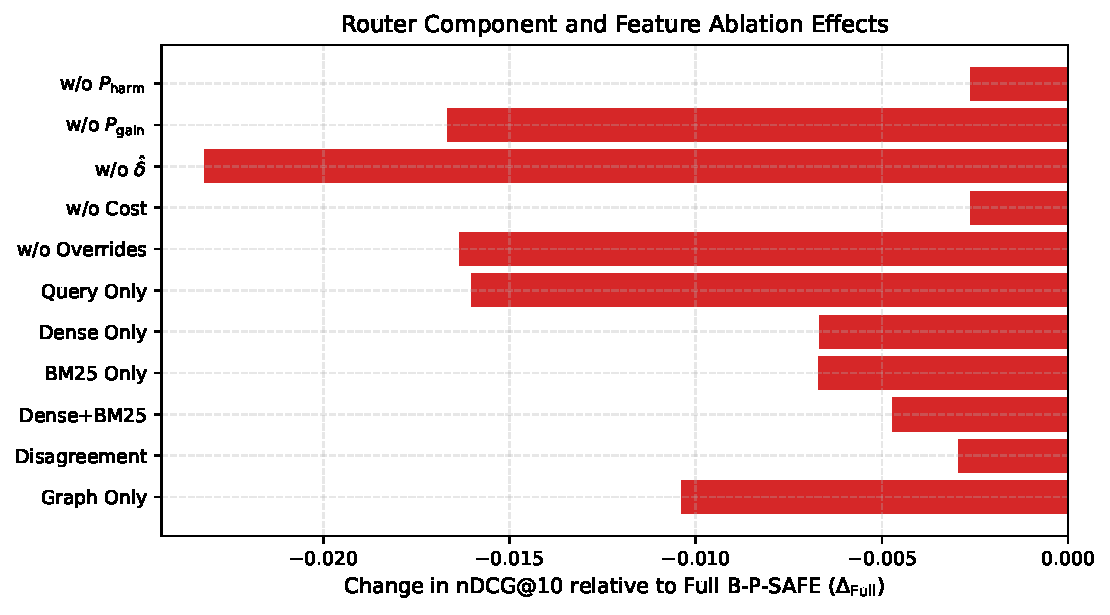
\includegraphics[width=0.48\textwidth]{fig9_ablation_matrix.pdf}
    \caption{Macro-average nDCG change ($\Delta_{\mathrm{Full}}$) across component and feature-group ablations.}
    \label{fig:ablations}
\end{figure}

Table~\ref{tab:ablations} and Fig.~\ref{fig:ablations} summarize the controlled ablation matrix. Full \bpsafe{} achieves top macro-average \ndcg{} ($0.4560$). Removing $P_{\mathrm{harm}}$ reduces harm avoidance and lowers mean quality. Among feature groups, lexical-dense disagreement signals (Jaccard overlap, rank correlation) and Dense score distributions contribute most strongly to routing efficacy.

\section{Discussion and Limitations}
\label{sec:discussion}

\subsection{Failure Case Analysis}
Inspection of per-query routing decisions reveals three diagnostic behaviors:
\begin{enumerate}
    \item \textbf{False Positives (Over-Escalation):} Queries where Dense retrieval was already optimal ($\text{nDCG}=1.0$), but high lexical specificity or moderate graph degree triggered unnecessary Cross-Encoder execution. Quality was preserved, but latency was incurred.
    \item \textbf{False Negatives (Under-Escalation):} Complex queries with subtle semantic vocabulary shifts where Dense score confidence was falsely elevated, causing the router to remain at Dense.
    \item \textbf{Harm Prevention Successes:} On ArguAna, BM25 keyword matching frequently dragged non-counterargument documents into the Cross-Encoder pool; \bpsafe{} successfully identified low gain and high harm risk, suppressing reranking on 85\% of queries.
\end{enumerate}

\subsection{Limitations}
\begin{itemize}
    \item \textbf{Binary Action Space:} The current verified release evaluates binary Dense-vs-Deep-Hybrid routing. Multi-tier intermediate routing (A0--A16) is documented in archive code and remains future work.
    \item \textbf{Hardware Dependence:} Latency savings are measured on a local NVIDIA RTX 5070 Ti GPU; distributed or CPU-only deployments may exhibit different latency profiles.
    \item \textbf{Safety Scope:} Safety in this work strictly refers to harm-aware protection against retrieval degradation ($\Delta\text{nDCG} < -0.01$). It does not evaluate adversarial robustness, jailbreak protection, or factual generation safety.
\end{itemize}

\section{Reproducibility Statement}
\label{sec:reproducibility}

All experiments, figures, and tables are fully reproducible from validated machine-readable artifacts. The repository includes an automated submission auditor:
\begin{verbatim}
python -m psafe.audit_submission
\end{verbatim}
which programmatically verifies all 18 submission criteria, data split disjointness, baseline completeness, and artifact provenance.

\section{Conclusion}
\bpsafe{} demonstrates that per-query risk- and cost-aware routing provides an effective, inspectable decision layer for retrieval cascades. Across four BEIR benchmarks, it achieves statistically validated quality gains over Dense, saves 20\%--66\% latency relative to always-on Deep Hybrid, prevents reranking harm on difficult corpora, and satisfies formal non-inferiority criteria.

\bibliographystyle{IEEEtran}
\bibliography{references}

\end{document}
